\documentclass[11pt]{article}
%\documentclass{foils}

\usepackage{koweydoc}
\usepackage{graphicx}
%\usepackage{koweyslide}
\newcommand{\commandline}{\texttt}
\newcommand{\commandgui}{\textit}

\begin{document}
\title{Geni Manual}
\author{Eric Kow\\LORIA}

\maketitle

\section{Introduction}

GenI is a surface realiser for natural language using 

\begin{itemize}
\item the Tree Adjoining Grammar (TAG) formalism 
\item a flat semantic representation
\item a head-driven generation algorithm
\end{itemize}

It runs on Linux and Mac OS X.  It might also run on Windows 
with a little work, but we have not tried.  

This document is in two major parts.  In section \ref{sec:walkthrough},
we give you a walkthrough of the basic functionality so you get an idea
of what the surface realiser does.  Sections \ref{sec:foo} to
\ref{sec:bar} provide much less handholding, but more detailed
information about using and configuration the realiser.  

\section{Walkthrough}

\subsection{Getting started}

You can run geni on the command line by executing the command 
\commandline{./geni} from your favourite terminal application.
What appears is the graphical interface\footnote{There is also
a non-interactive text version of the interface, see section 
\ref{sec:configuration_files}}:

% this is how you would include an image in your document
\begin{figure}[h]
\begin{center}
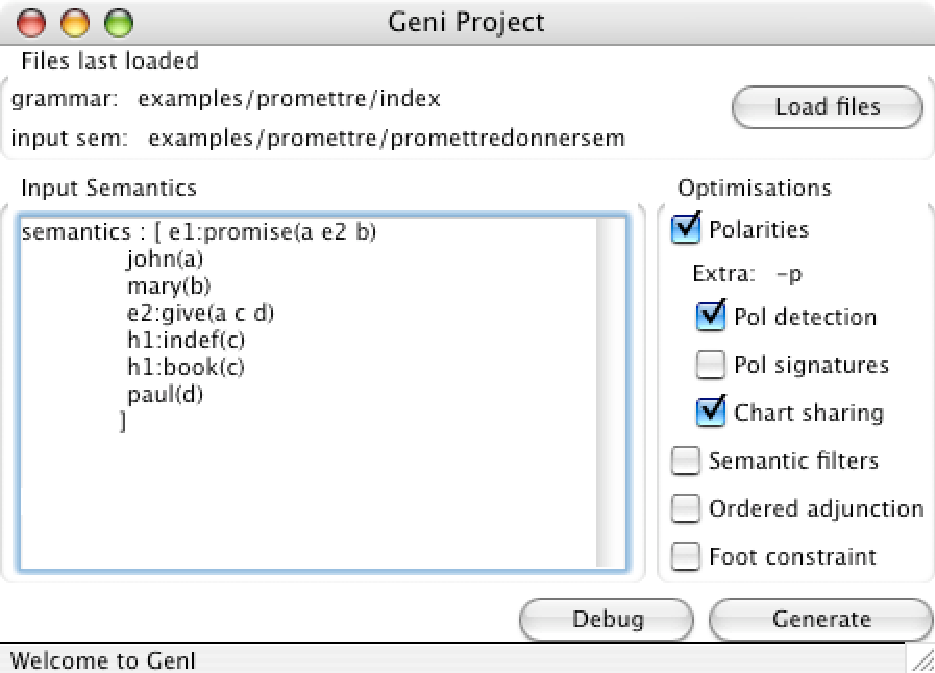
\includegraphics[scale=0.75]{images/geni_gui.pdf}
\label{fig:geni_screenshot}
\end{center}
\end{figure}

The surface realiser takes two inputs: a grammar and a semantic
expression. GenI provides a default grammar and semantics, so
let's take a look at what these inputs produce: click on the 
\commandgui{Generate} button.

What appears, maybe after some seconds of thinking is a results window.
To the see the output, click on the \commandgui{Realisations} tab:  

% this is how you would include an image in your document
\begin{figure}[h]
\begin{center}
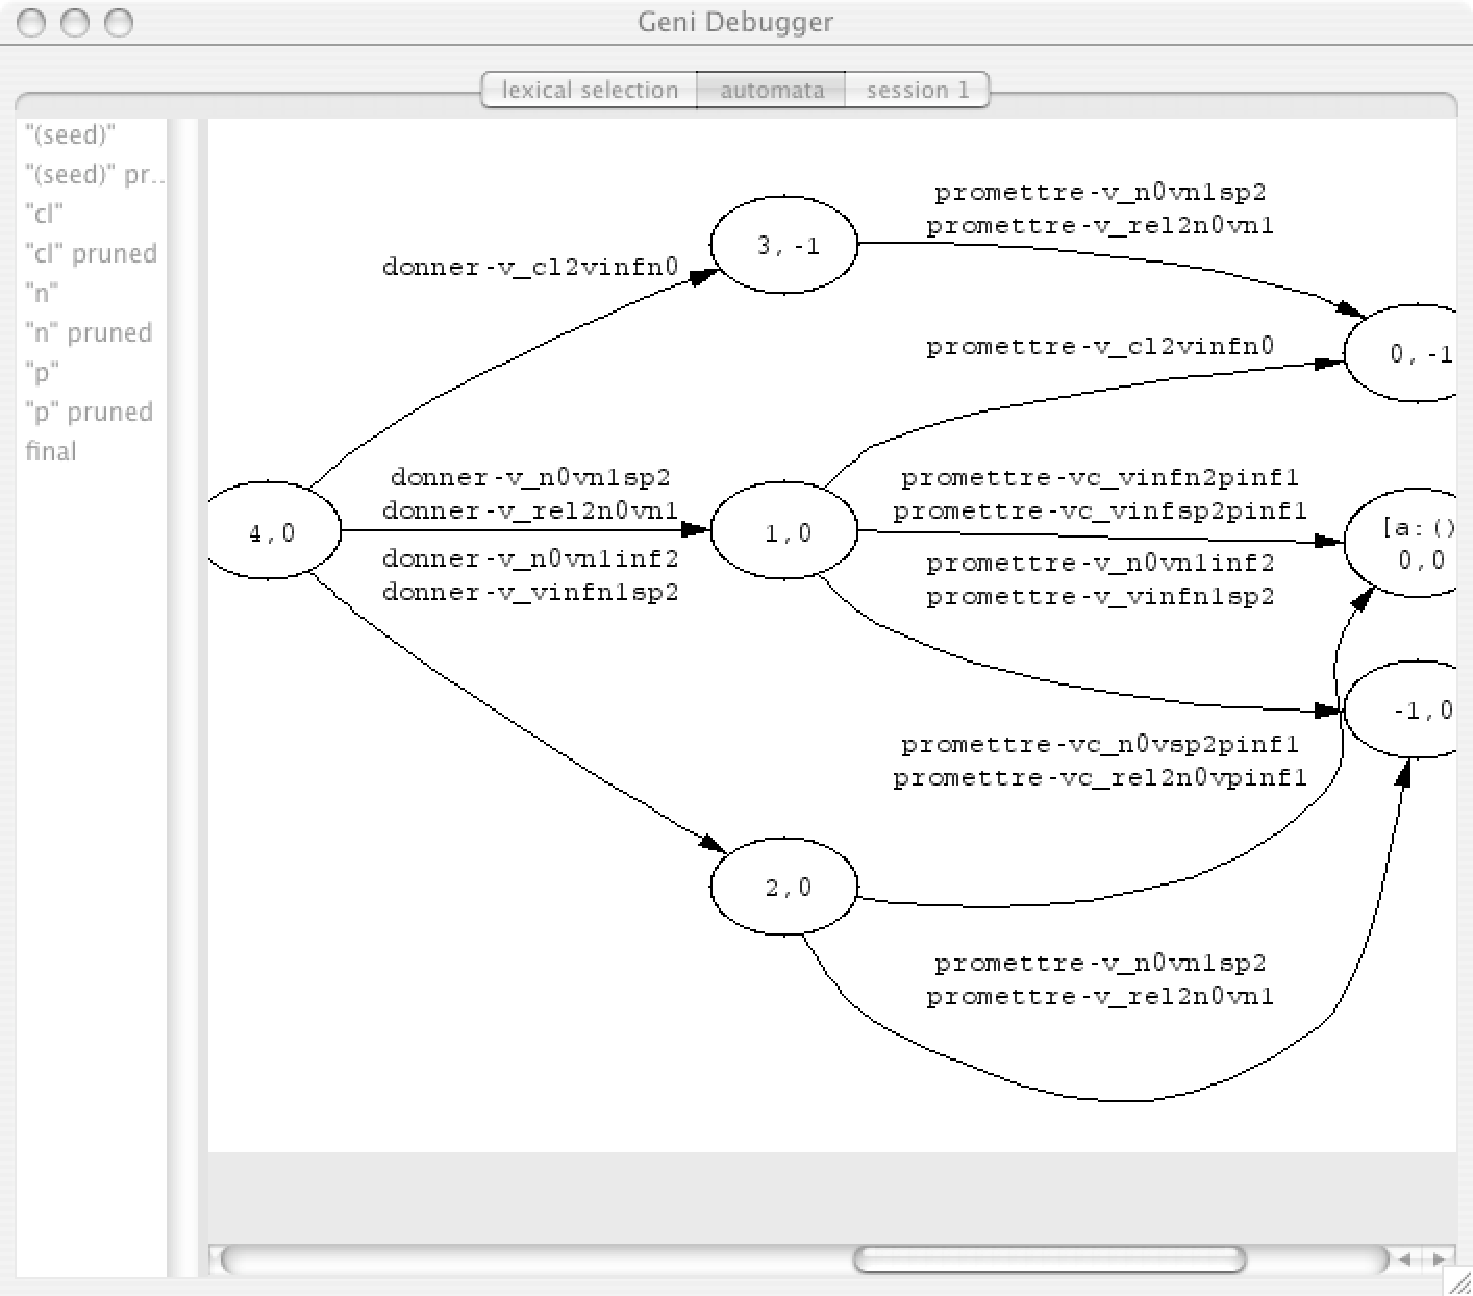
\includegraphics[scale=0.75]{images/geni_polaut.pdf}
\label{fig:geni_results}
\caption{Results: Realisations tab}
\end{center}
\end{figure}

You should see a small number of sentences on the left. If you click on
one of these sentences, its derivation and derived tree will appear on
the right.

Summary so far:

\begin{enumerate}
\item \commandline{./geni}
\item click on \commandgui{Generate}
\item results window: click on \commandgui{Realisations}
\end{enumerate}

Voila! This shows you roughly the kind of things GenI is capable of
doing.  Now in the rest of the walkthrough, we'll see how the realiser
responds to a different input semantics and grammar.

\subsection{Input semantics}

You write the input semantics without any commas:
\begin{verbatim}
\end{verbatim}

You can also specify handles in the semantics:
\begin{verbatim}
\end{verbatim}

Or write recursively embedded semantics:
\begin{verbatim}
\end{verbatim}

But if you add handles, please be sure to add them to every literal,
or GenI could behave unpredicatably.

\subsection{Grammar}

%:
%
%% this is how you would include an image in your document
%\begin{figure}[h]
%\begin{center}
%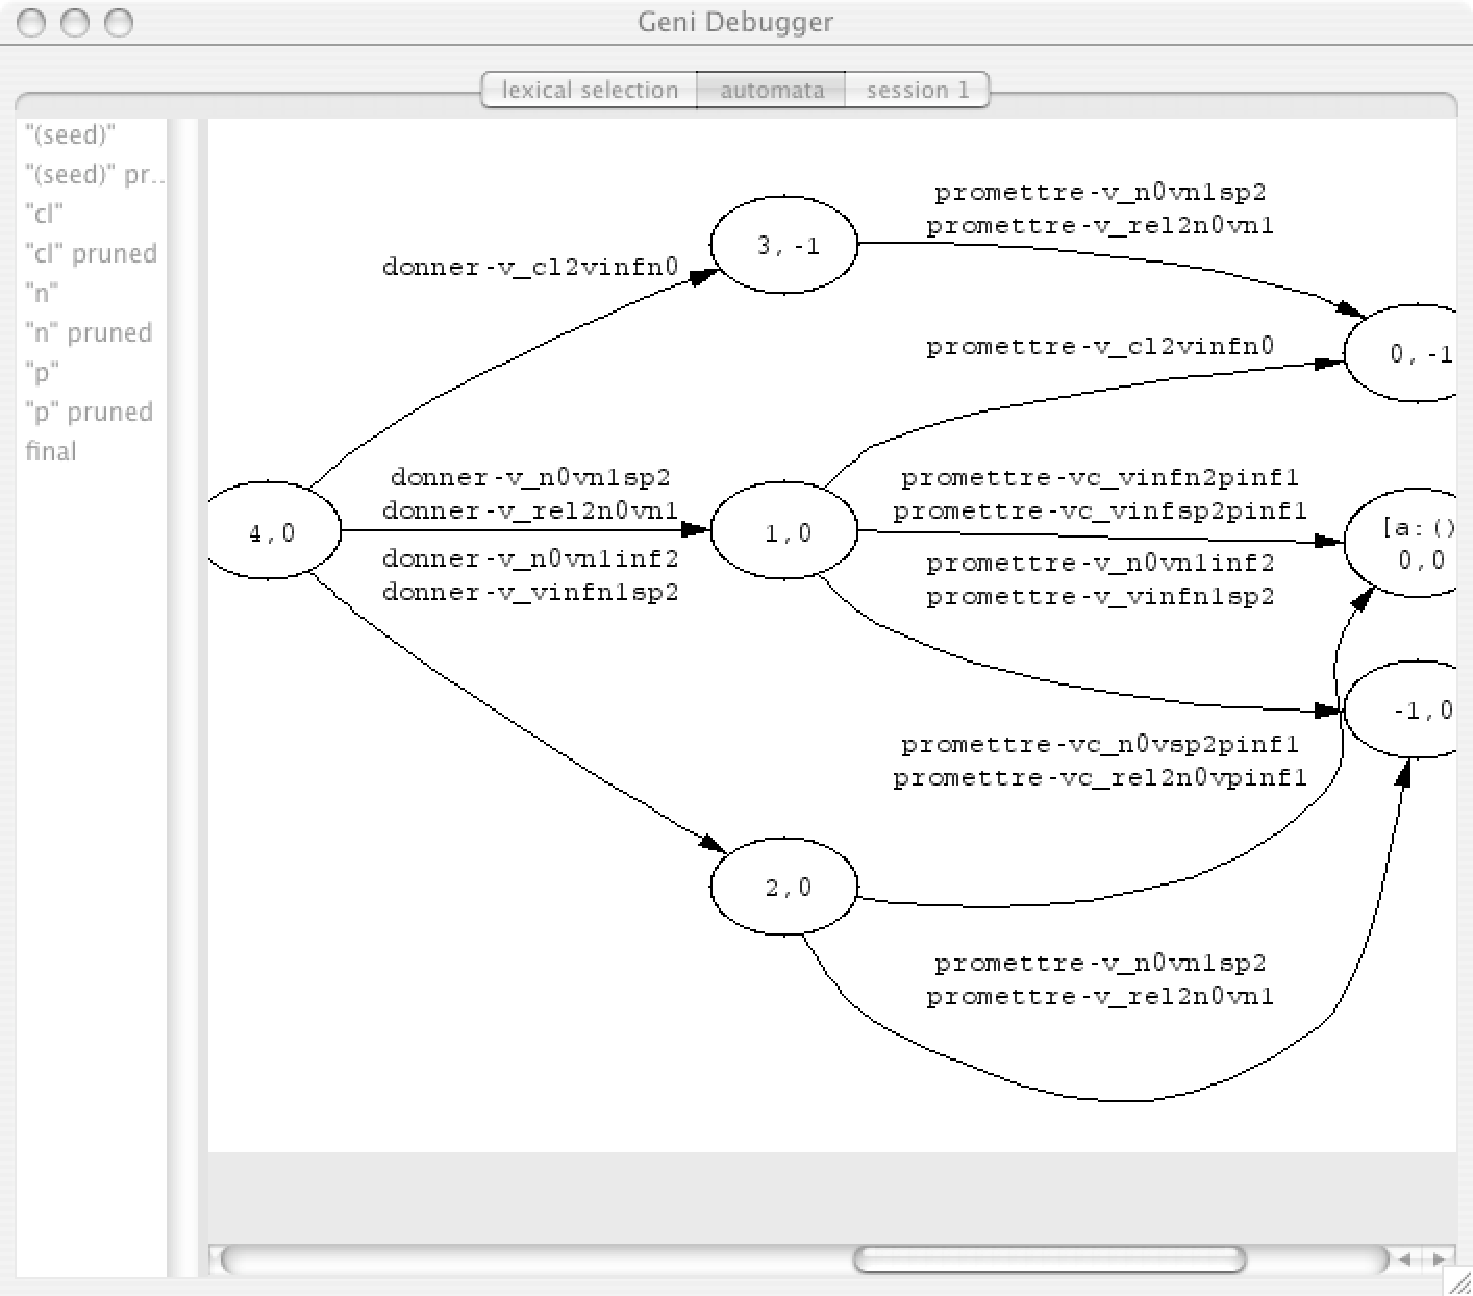
\includegraphics[scale=0.75]{images/geni_polaut.pdf}
%\label{fig:geni_results}
%\caption{Results: Lexical selection}
%\end{center}
%\end{figure}
%
%What you see here is the lexical selection tab.  It shows you the subset
%of the grammar that GenI used for realisation of the input semantics.

\section{Configuration files}
\label{sec:configuration_files}

GenI configuration consists of a list of
attributes and values of the form Attribute = Value.  For example: 

\begin{verbatim}
Macros   = chatnoirmac
Lexicon  = chatnoirlex
TSemantics = chatnoirsem
\end{verbatim}

The basic configuration attributes are

\begin{description}
\item[Macros, Lexicon] files for the Geni grammar
\item[GrammarXml]      files for the Geni grammar as XML (note: if this
                       is set, Macros/Lexicon will be ignored)
\item[TSemantics]      file containing an input semantics
\item[Optimisations]   a comma delimited list of optimisations (see
                       section \ref{sec:optimisations}).
\item[ExtraPolarities] a list of default polarities for paraphrase selection   
\end{description}

\subsection{Optimisations}

For a more thorough description of these optimisations, see
\cite{kow2003}.

\subsubsection{Polarity automata}

The first set of optimisations is to filter the lexical selection,
so that only (potentially) syntactically compatible combinations
of trees are given to the generator.  

\begin{description}
\item[Polarised] construct polarity automata at all
\item[PolSig]    group trees into polarity signatures, i.e. by their
                 semantics and polarities
\item[PolSort]   when constructing the automaton, first sort the
                 literals of the target semantics by the number
                 of trees which correspond to that literal
\item[ChartSharing] instead of performing a seperate realisation
                    for each automaton path, annotate the trees
                    with their path information and only compare
                    trees on an intersecting set of paths
\end{description}

\subsubsection{Adjunction}

The other optimisations deal with the adjunction phase of the
generator.

\begin{description}
\item[SemFiltered] before passing to the adjunction phase,
                   first filter out the trees which we know
                   will be semantically incomplete.
\item[OrderedAdj] impose an order on which potential
                  adjunction nodes of a tree are explored
\item[FootConstraint] do not allow the foot node of an auxiliary tree to
                      become an adjunction node after it has been 
                      adjoined into a tree
\end{description}

\subsection{Batch processing}
There are two types of batch processing:
\begin{enumerate}
\item Multi-input:
      You can write multiple configurations in .genirc if you separate
      them by a bang (!).  This will run geni in multiple sessions.
      Each session inherits the configuration of the previous session,
      except for the attributes that you overwrite.  Don't forget to
      unset your ExtraPolarities or Optimisations unless you want them
      to be inherited!
\item Optimisations = Batch 
      Will run geni through all the possible combinations of
      optimisations.  This is useful for performance testing
      of the GenI optimisations
      N.B. you can use Optimisations=Batch together with multi-input
      if you want.
\end{enumerate}

\section{Grammar files}

\subsection{Hand-written grammars}

\subsubsection{Polarities}

Polarities mainly go in the macros file.  They appear in the optional
second parenthesis like so:

\begin{verbatim}
  IntrV(Event Agent ! agr:A) (+np +np)
\end{verbatim}

Examples of polarities: +foo, -foo, +3foo, or -3foo

\subsubsection{TAGML from MGC}

There seems to be no convention for indicating how inflected 
forms are placed in TAGML tree.  Until somebody tells me 
otherwise, I am going with the following

\begin{verbatim}
<node type="none">
  <fs>
    <f name="phon">foo</f>
  </fs>
</node>
\end{verbatim}

I refuse to change this until you show me something vaguely
official-looking.


\section{Conclusion}

% this is how you would include an image in your document
%\begin{figure}
%\begin{center}
%\includegraphics{images/foo.pdf}
%\end{center}
%\end{figure}




\end{document}
